\chapter{Probl\`emes d'int\'egration des \'equations du mouvement}

\section{Mouvement lin\'eaire}

\subsection{Oscillations d'un pendule math\'ematique plan}

\begin{figure}[htb!]
	\begin{center}
		\begin{picture}(100,100)(0,0)
			%axis
			\linethickness{0.05mm}
			\multiput(0,100)(10,0){10}{\line(1,0){8}}\put(102,95){$x$}
			\multiput(0,0)(0,10){10}{\line(0,1){8}}\put(-5,-10){$y$}
			%socle
			\put(0,100){\color{black}\circle*{5}}
			%arms
			\linethickness{0.5mm}
			\put(0,100){\line(10,-15){70}}
			\put(40,50){$l$}
			\put(68,-5){\color{black}\circle*{10}}\put(75,-7){$m$}
			%angles
			\linethickness{0.05mm}
			\qbezier(0,80),(5,82),(10,85)
			\put(3,70){$\varphi$}
		\end{picture}
		\caption{Pendule double oscillant}\label{FIG:3_1_1}
	\end{center}
\end{figure}

Il s'agit de trouver la p\'eriode d'oscillation du pendule en fonction de l'amplitude du mouvement. En supposant $\varphi_{0}$ l'angle maximal par rapport \`a la verticale, o\`u la vitesse du pendule est nulle, l'\'energie totale du pendule est :
\bea
	E & = & \frac{m}{2}\left[\dfrac{\mathrm{d}(l\varphi)}{\mathrm{dt}}\right]^{2} - mgl\cos\varphi \nonumber \\
	& = & \frac{m}{2}l^{2}\dot{\varphi}^{2} - mgl\cos\varphi
\eea
et par conservation de l'\'energie totale :
\be
	E = E(\varphi_{0}) = -mgl\cos\varphi_{0}
\ee
Par sym\'etrie du mouvement, la p\'eriode est \'egale au temps de parcours entre $\varphi=0$ et $\varphi=\varphi_{0}$. Sachant que la quantit\'e, $E-U$ vaut $-mgl\cos\varphi_{0} + mgl\cos\varphi$, l'\'equation (\ref{EQ:11_3}) peut s'\'ecrire :
\bea
	\mathrm{T} & = & 4\sqrt{\frac{m}{2}}\int_{0}^{\varphi_{0}}{\dfrac{\mathrm{d}(l\varphi)}{\sqrt{mgl(\cos\varphi - \cos\varphi_{0})}}} \nonumber \\
	& = & 4\sqrt{\frac{l}{2g}}\int_{0}^{\varphi_{0}}{\dfrac{\mathrm{d}\varphi}{\sqrt{\cos\varphi - \cos\varphi_{0}}}}
\eea
Notons que :
\bea
	\sin^{2}\frac{\alpha}{2} & = & \left(\dfrac{e^{i\frac{\alpha}{2}} - e^{-i\frac{\alpha}{2}}}{2i}\right)^{2} \nonumber \\
	& = & -\frac{1}{4}\left(e^{i\alpha} + e^{-i\alpha} - 2e^{i\frac{\alpha}{2}-i\frac{\alpha}{2}}\right) \nonumber \\
	& = & -\frac{1}{4}\left(e^{i\alpha} + e^{-i\alpha} - 2\right) \nonumber \\
	& = & \frac{1}{2}\left(1-\cos\alpha\right) \nonumber \\
	\Leftrightarrow \cos\alpha & = & 1 - 2\sin^{2}\frac{\alpha}{2}
\eea
Cela permet de d\'evelopper la p\'eriode telle que :
\bea
	\mathrm{T} & = & 4\sqrt{\frac{l}{2g}}\int_{0}^{\varphi_{0}}{\dfrac{\mathrm{d}\varphi}{\sqrt{1-2\sin\frac{\varphi}{2} - 1 + \sin\frac{\varphi_{0}}{2}}}} \nonumber \\
	& = & 4\sqrt{\frac{l}{2g}}\int_{0}^{\varphi_{0}}{\dfrac{\mathrm{d}\varphi}{\sqrt{2\left(\sin\frac{\varphi_{0}}{2} - \sin\frac{\varphi}{2}\right)}}} \nonumber \\
	& = & 2\sqrt{\frac{l}{g}}\int_{0}^{\varphi_{0}}{\dfrac{\mathrm{d}\varphi}{\sqrt{\sin\frac{\varphi_{0}}{2} - \sin\frac{\varphi}{2}}}}
\eea
En posant $\sin\xi = \dfrac{\sin(\varphi/2)}{\sin(\varphi_{0}/2)}$, nous avons pour $\varphi = 0$, $\sin\xi = 0$ soit $\xi = 0$ et pour $\varphi = \varphi_{0}$, $\sin\xi = 1$ soit $\xi = \frac{\pi}{2}$. En d\'eveloppant la d\'efinition de $\sin\xi$ pour l'inverser, nous trouvons :
\bea
	\sin^{2}\xi\sin^{2}\left(\frac{\varphi_{0}}{2}\right) & = & \sin^{2}\left(\frac{\varphi}{2}\right) \nonumber \\
	& = & 1 - \cos^{2}\left(\frac{\varphi}{2}\right) \nonumber \\
	\Leftrightarrow \cos\left(\frac{\varphi}{2}\right) & = & \sqrt{1 - \sin^{2}\left(\frac{\varphi_{0}}{2}\right)\sin^{2}\xi}
\eea
et pour conna\^itre la correspondance entre $\mathrm{d}\varphi$ et $\mathrm{d}\xi$ :
\bea
	\sin\xi & = & \dfrac{\sin\left(\frac{\varphi}{2}\right)}{\sin\left(\frac{\varphi_{0}}{2}\right)} \nonumber \\
	\Leftrightarrow \cos\xi\mathrm{d}\xi & = & \dfrac{\cos\left(\frac{\varphi}{2}\right)}{2\sin\left(\frac{\varphi_{0}}{2}\right)}\mathrm{d}\varphi \nonumber \\
	\mathrm{d}\varphi & = & \dfrac{2\sin\left(\frac{\varphi_{0}}{2}\right)\cos\xi}{\cos\left(\frac{\varphi}{2}\right)}\mathrm{d}\xi \nonumber \\
	& = & \dfrac{2\sin\left(\frac{\varphi_{0}}{2}\right)\sqrt{1 - \sin^{2}\xi}}{\cos\left(\frac{\varphi}{2}\right)}\mathrm{d}\xi \nonumber \\
	& = & \dfrac{2\sin\left(\frac{\varphi_{0}}{2}\right)\sqrt{1 - \dfrac{\sin^{2}\left(\frac{\varphi}{2}\right)}{\sin^{2}\left(\frac{\varphi_{0}}{2}\right)}}}{\cos\left(\frac{\varphi}{2}\right)}\mathrm{d}\xi \nonumber \\
	& = & \dfrac{2\sqrt{\sin^{2}\left(\frac{\varphi_{0}}{2}\right) - \sin^{2}\left(\frac{\varphi}{2}\right)}}{\cos\left(\frac{\varphi}{2}\right)}\mathrm{d}\xi \nonumber \\
	\Leftrightarrow \dfrac{\mathrm{d}\varphi}{\sqrt{\sin^{2}\left(\frac{\varphi_{0}}{2}\right) - \sin^{2}\left(\frac{\varphi}{2}\right)}} & = & \dfrac{2\mathrm{d}\xi}{\sqrt{1 - \sin^{2}\left(\frac{\varphi_{0}}{2}\right)\sin^{2}\xi}}
\eea
En cons\'equence, en posant :
\be
	K(k) = \int_{0}^{\frac{\pi}{2}}\dfrac{\mathrm{d}\xi}{\sqrt{1 - k^{2}\sin^{2}\xi}}
\ee
la p\'eriode $\mathrm{T}$ se r\'e\'ecrit ainsi\footnote{Dans le livre, il est indiqu\'e que l'argument de la fonction $K$ est $\frac{\sin\left(\varphi_{0}\right)}{2}$, je pense qu'il ne s'agit que d'une coquille.} :
\be
	\mathrm{T} = 4\sqrt{\dfrac{l}{g}}K\left(\sin(\varphi_{0}/2)\right)
\ee
La fonction $K$ est l'int\'egrale elliptique compl\`ete de premi\`ere esp\`ece. Elle admet comme d\'eveloppement en s\'erie enti\`ere :
\bea
	K(k) & = & \dfrac{\pi}{2}\sum_{n=0}^{+\infty}\left[\dfrac{(2n)!}{2^{2n}(n!)^{2}}\right]^{2}k^{2n} \nonumber \\
	& =& \dfrac{\pi}{2}\left(1 + \left(\dfrac{2}{4 \times 1}\right)^{2}k^{2} + \cdots\right)
\eea
donc pour de petites oscillations telles que $\sin(\varphi_{0}/2)\simeq\varphi_{0}/2\ll 1$ :
\be
	K(\sin\varphi_{0}/2) = \dfrac{\pi}{2}\left(1 + \dfrac{1}{16}\varphi_{0}^{2} + \cdots\right)
\ee
soit :
\be
	\mathrm{T} = 2\pi\sqrt{\dfrac{l}{g}}\left(1 + \dfrac{1}{16}\varphi_{0}^{2} + \cdots\right)
\ee
et en premi\`ere approximation, la p\'eriode du mouvement n'est d\'ependante ni de la masse de la particule ni de l'amplitude initiale.

\subsection{Cas d'\'energies potentielles particuli\`eres}

Il s'agit de d\'eterminer la p\'eriode d'oscillations en fonction de l'\'energie pour le mouvement d'une particule de masse $m$ dans un champ o\`u l'\'energie potentielle $U$ est d\'efinie telle que :

\subsubsection{$U = A\lvert x \rvert^{n}$}

\begin{figure}[htb!]
	\begin{center}
		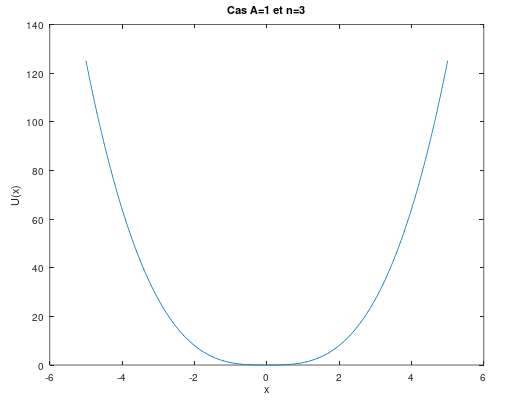
\includegraphics[width=10cm]{chapter_03_exercice_2a}
		\caption{$U = \lvert x \rvert^{n}$ pour $n \in \{1,2,3,4,5\}$}\label{FIG:3_2_a}
	\end{center}
\end{figure}

Dans ce cas pr\'ecis, commen\c{c}ons par d\'efinir les points d'arr\^et tels que $E=U$, soit $x = \pm\left(\dfrac{E}{A}\right)^{\frac{1}{n}}$. Cela permet d'\'ecrire l'\'equation (\ref{EQ:11_5}) telle que :
\bea
	\mathrm{T}(E) & = & \sqrt{2m}\int_{-\left(\frac{E}{A}\right)^{\frac{1}{n}}}^{+\left(\frac{E}{A}\right)^{\frac{1}{n}}}\dfrac{\mathrm{d}x}{\sqrt{E - A\lvert x \rvert^{n}}} \nonumber \\
	& = & 2\sqrt{2m}\int_{0}^{+\left(\frac{E}{A}\right)^{\frac{1}{n}}}\dfrac{\mathrm{d}x}{\sqrt{E - Ax^{n}}} \nonumber \\
	& = & 2\sqrt{\dfrac{2m}{E}}\int_{0}^{+\left(\frac{E}{A}\right)^{\frac{1}{n}}}\dfrac{\mathrm{d}x}{\sqrt{1 - \dfrac{Ax^{n}}{E}}}
\eea
car la fonction $U$ est paire, i.e. $U(x) = U(-x)$. En posant :
\be
	y = \left(\dfrac{A}{E}\right)^{\frac{1}{n}}x
\ee
qui permet d'\'ecrire :
\be
	\begin{cases}
		y^{n} = \dfrac{A}{E}x^{n} \\
		\mathrm{d}y = \left(\dfrac{A}{E}\right)^{\frac{1}{n}}\mathrm{d}x
	\end{cases}
\ee
et :
\be
	\begin{cases}
		x = 0 \Rightarrow y = 0 \\
		x = \left(\dfrac{E}{A}\right)^{\frac{1}{n}} \Rightarrow y = \left(\dfrac{A}{E}\right)^{\frac{1}{n}}\left(\dfrac{E}{A}\right)^{\frac{1}{n}} = 1
	\end{cases}
\ee
La p\'eriode $\mathrm{T}$ devient :
\bea
	\mathrm{T} & = & 2\sqrt{\dfrac{2m}{E}}\int_{0}^{1}\left(\dfrac{E}{A}\right)^{\frac{1}{n}}\dfrac{\mathrm{d}y}{\sqrt{1 - y^{n}}} \nonumber \\
	& = & 2\dfrac{\sqrt{2mE^{\frac{1}{n}-\frac{1}{2}}}}{A^{\frac{1}{n}}}\int_{0}^{1}\dfrac{\mathrm{d}y}{\sqrt{1 - y^{n}}}
\eea
De la m\^eme mani\`ere, en posant $u=y^{n}$, nous avons :
\be
	\begin{cases}
		y = 0 \Rightarrow u = 0 \\
		y = 1 \Rightarrow u = 1
	\end{cases}
\ee
ainsi que :
\be
	\begin{cases}
		y = u^{\frac{1}{n}} \Rightarrow y^{n-1} = u^{\frac{n-1}{n}} = u^{1 - \frac{1}{n}} \\
		ny^{n-1}\mathrm{d}y = \mathrm{d}u \Leftrightarrow \mathrm{d}y = \dfrac{u^{\frac{1}{n} - 1}}{n}\mathrm{d}u
	\end{cases}
\ee
Nous arrivons \`a :
\bea
	\mathrm{T} & = & 2\dfrac{\sqrt{2m}E^{\frac{1}{n}-\frac{1}{2}}}{A^{\frac{1}{n}}}\int_{0}^{1}\dfrac{u^{\frac{1}{n} - 1}\mathrm{d}u}{n(1-u)^{\frac{1}{2}}} \nonumber \\
	& = & 2\dfrac{\sqrt{2m}E^{\frac{1}{n}-\frac{1}{2}}}{nA^{\frac{1}{n}}}\int_{0}^{1}u^{\frac{1}{n} - 1}(1-u)^{\frac{-1}{2}}\mathrm{d}u \label{EQ:APP3_2_a}
\eea
Utilisons ici les int\'egrales d'Euler de premi\`ere esp\`ece, \emph{fonction Béta}, d\'efinies telles que :
\be
	\mathrm{B}(x,y) = \int_{0}^{1}\mathrm{t}^{x-1}(1-\mathrm{t})^{y-1}\mathrm{dt} = \dfrac{\Gamma(x)\Gamma(y)}{\Gamma(x+y)} \label{EQ:INT_EULER_BETA}
\ee
et celles de seconde esp\`ece, \emph{fonction Gamma} :
\be
	\Gamma(z) = \int_{0}^{+\infty}\mathrm{t}^{z-1}e^{-\mathrm{t}}\mathrm{dt} \label{EQ:INT_EULER_GAMMA}
\ee
L'\'equation (\ref{EQ:APP3_2_a}) s'\'ecrit alors :
\bea
	\mathrm{T} & = & 2\dfrac{\sqrt{2m}E^{\frac{1}{n}-\frac{1}{2}}}{nA^{\frac{1}{n}}}\mathrm{B}\left(\frac{1}{n},\frac{1}{2}\right) \nonumber \\
	& = & 2\dfrac{\sqrt{2m}E^{\frac{1}{n}-\frac{1}{2}}}{nA^{\frac{1}{n}}}\dfrac{\Gamma\left(\frac{1}{n}\right)\Gamma\left(\frac{1}{2}\right)}{\Gamma\left(\frac{1}{n}+\frac{1}{2}\right)} \nonumber
\eea
Or $\Gamma(1/2) = \sqrt{\pi}$, nous avons donc finalement :
\be
	\mathrm{T} = 2\dfrac{\sqrt{2\pi m}\Gamma\left(\frac{1}{n}\right)}{nA^{\frac{1}{n}}\Gamma\left(\frac{1}{n}+\frac{1}{2}\right)}E^{\frac{1}{n}-\frac{1}{2}}
\ee

\begin{figure}[htb!]
	\begin{center}
		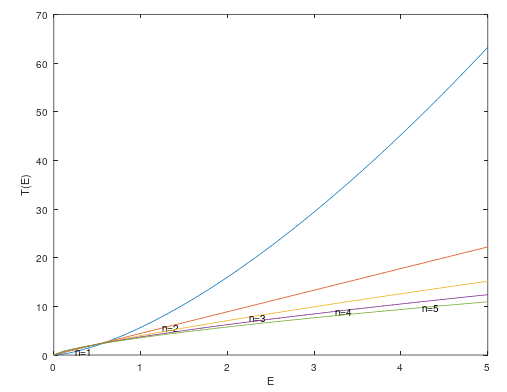
\includegraphics[width=10cm]{chapter_03_exercice_2a_result}
		\caption{$\mathrm{T}(E)$ pour $m=1$, $A=1$ et $n \in \{1,2,3,4,5\}$}\label{FIG:3_2_a_result}
	\end{center}
\end{figure}

\subsubsection{$U = -U_{0}/\cosh^{2}(\alpha x)$ avec $-U_{0} < E < 0$}

\begin{figure}[htb!]
	\begin{center}
		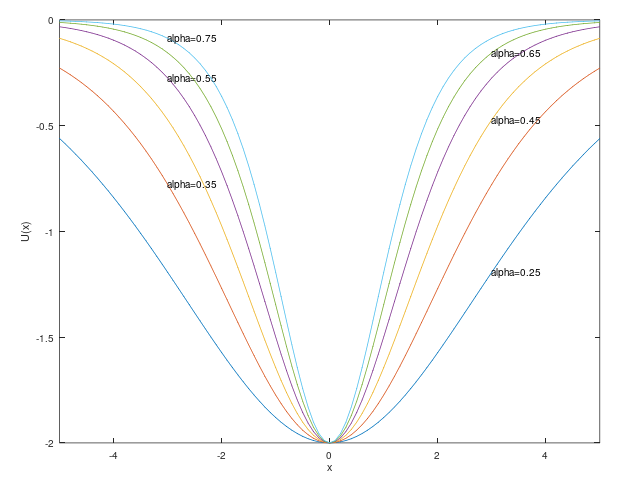
\includegraphics[width=10cm]{chapter_03_exercice_2b}
		\caption{$U = -2 / \cosh^{2}(\alpha x)$ pour $\alpha \in \{0.25,0.35,0.45,0.55,0.65,0.75\}$}\label{FIG:3_2_b}
	\end{center}
\end{figure}

Les point d'arr\^et sont toujours d\'efinis tels que $U=E$, i.e. :
\bea
	\cosh^{2}(\alpha x) & = & -\dfrac{U_{0}}{E} \nonumber \\
	\Leftrightarrow \alpha x & = & \pm \arccosh\left(\sqrt{\dfrac{-U_{0}}{E}}\right)
\eea
Ceci est possible car $-U_{0} < E < 0$ et donc $-U_{0}/E > 0$. Les points d'arr\^et sont donc :
\be
	x = \pm \dfrac{1}{\alpha}\arccosh\left(\sqrt{\dfrac{-U_{0}}{E}}\right)
\ee

L'\'equation (\ref{EQ:11_5}) peut donc s'\'ecrire :
\bea
	\mathrm{T}(E) & = & \sqrt{2m}\int_{-\frac{1}{\alpha}\arccosh\left(\sqrt{\frac{-U_{0}}{E}}\right)}^{\frac{1}{\alpha}\arccosh\left(\sqrt{\frac{-U_{0}}{E}}\right)}\dfrac{\mathrm{d}x}{\sqrt{E + \dfrac{U_{0}}{\cosh^{2}(\alpha x)}}} \nonumber \\
	& = & \sqrt{\dfrac{2m}{\lvert E \rvert}}\int_{-\frac{1}{\alpha}\arccosh\left(\sqrt{\frac{-U_{0}}{E}}\right)}^{\frac{1}{\alpha}\arccosh\left(\sqrt{\frac{-U_{0}}{E}}\right)}\dfrac{\mathrm{d}x}{\sqrt{1 + \dfrac{U_{0}}{E\cosh^{2}(\alpha x)}}}
\eea
car $E < 0$. En choisissant :
\be
	y = \sqrt{\frac{-U_{0}}{E}}\dfrac{1}{\cosh(\alpha x)}
\ee
nous obtenons pour les bornes de l'int\'egrale :
\be
	\begin{cases}
		x = -\frac{1}{\alpha}\arccosh\left(\sqrt{\frac{-U_{0}}{E}}\right) \Rightarrow y = -1 \\
		x = \frac{1}{\alpha}\arccosh\left(\sqrt{\frac{-U_{0}}{E}}\right) \Rightarrow y = 1 \\
	\end{cases}
\ee
et :
\bea
	y^{2} & = & \frac{-U_{0}}{E}\dfrac{1}{\cosh^{2}(\alpha x)} \nonumber \\
	\mathrm{d}y & = & \sqrt{\frac{-U_{0}}{E}}\dfrac{-\alpha}{\cosh^{2}(\alpha x)}\mathrm{d}x \nonumber \\
	\Leftrightarrow & = & -\alpha\sqrt{\frac{-U_{0}}{E}}\dfrac{E}{-U_{0}}y^{2}\mathrm{d}x \nonumber \\
	\Leftrightarrow \mathrm{d}x & = & -\sqrt{\frac{-U_{0}}{E}}\dfrac{\mathrm{d}y}{\alpha y^{2}}
\eea
La p\'eriode s'\'ecrit alors :
\bea
	\mathrm{T}(E) & = & \sqrt{\dfrac{2m}{\lvert E \rvert}}\int_{-1}^{1}\dfrac{y^{-2}\mathrm{d}y}{\sqrt{1-y^{2}}}\times \dfrac{-1}{\alpha}\sqrt{\dfrac{-U_{0}}{E}} \nonumber \\
	& = & -\dfrac{2}{\alpha}\sqrt{\dfrac{-U_{0}}{E}}\sqrt{\dfrac{2m}{\lvert E \rvert}}\int_{0}^{1}\dfrac{y^{-2}\mathrm{d}y}{\sqrt{1-y^{2}}}
\eea

En posant $u = y^{2}$, soit $y = u^{1/2}$ et $\mathrm{d}u = 2y\mathrm{d}y = 2u^{1/2}\mathrm{d}y \Leftrightarrow \mathrm{d}y = \frac{1}{2}u^{-1/2}\mathrm{d}u$, alors la p\'eriode devient :
\bea
	\mathrm{T}(E) & = & -\dfrac{2}{\alpha}\sqrt{\dfrac{-U_{0}}{E}}\sqrt{\dfrac{2m}{\lvert E \rvert}}\int_{0}^{1}\frac{1}{2}\dfrac{u^{-3/2}\mathrm{d}u}{(1-u)^{1/2}} \nonumber \\
	& = & -\dfrac{1}{\alpha}\sqrt{\dfrac{-U_{0}}{E}}\sqrt{\dfrac{2m}{\lvert E \rvert}} \mathrm{B}\left(-\frac{1}{2},\frac{1}{2}\right) \nonumber \\
	& = & \dfrac{2\pi}{\alpha}\sqrt{\dfrac{-U_{0}}{E}}\sqrt{\dfrac{2m}{\lvert E \rvert}}
\eea
car $\Gamma(0) = 1$, $\Gamma(\frac{1}{2}) = \sqrt{\pi}$ et $\Gamma(-\frac{1}{2}) = -2\sqrt{\pi}$. Ici, je trouve une solution diff\'erente de celle propos\'ee par le livre qui est : $\mathrm{T}(E) = \dfrac{\pi}{\alpha}\sqrt{\dfrac{2m}{\lvert E \rvert}}$ et j'avoue ne pas savoir en quoi la p\'eriode ne pourrait pas d\'ependre de la profondeur du puits d'\'energie potentielle $U_{0}$.

\subsubsection{$U = U_{0}\tan^{2}(\alpha x)$}

Tout d'abord quelques rappels sur la fonction \emph{tangente} :
\bea
	\tan\alpha & = & \dfrac{\sin\alpha}{\cos\alpha} = \dfrac{e^{i\alpha} - e^{-i\alpha}}{i(e^{i\alpha} + e^{-i\alpha})} \nonumber \\
	\tan'\alpha & = & \dfrac{1}{\cos^{2}\alpha} = 1 + \tan^{2}\alpha
\eea

\begin{figure}[htb!]
	\begin{center}
		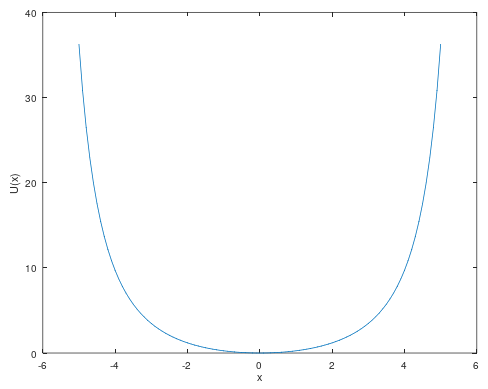
\includegraphics[width=10cm]{chapter_03_exercice_2c}
		\caption{$U = 4\tan^{2}(\alpha x)$ pour $\alpha \in \{0.25,0.35,0.45,0.55,0.65,0.75\}$}\label{FIG:3_2_c}
	\end{center}
\end{figure}

Les points d'arr\^et du mobile sont d\'efinis tels que $U = E = U_{0}\tan^{2}(\alpha x)$, soit $\tan(\alpha x) = \pm\sqrt(E/U_{0})$ :
\be
	\begin{cases}
		x_{1} = -\frac{1}{\alpha}\arctan\left(\sqrt{\dfrac{E}{U_{0}}}\right) \\
		x_{2} = +\frac{1}{\alpha}\arctan\left(\sqrt{\dfrac{E}{U_{0}}}\right)
	\end{cases}
\ee
car la fonction $\arctan$ est impaire. Par cons\'equence, la p\'eriode $\mathrm{T}$ s'\'ecrit \`a partir de l'\'equation (\ref{EQ:11_5}) :
\bea
	\mathrm{T}(E) & = & \sqrt{2m}\int_{-\frac{1}{\alpha}\arctan\left(\sqrt{\frac{E}{U_{0}}}\right)}^{\frac{1}{\alpha}\arctan\left(\sqrt{\frac{E}{U_{0}}}\right)}\dfrac{\mathrm{d}x}{\sqrt{E - U_{0}\tan^{2}(\alpha x)}} \nonumber \\
	& = & 2\sqrt{\dfrac{2m}{E}}\int_{0}^{\frac{1}{\alpha}\arctan\left(\sqrt{\frac{E}{U_{0}}}\right)}\dfrac{\mathrm{d}x}{\sqrt{1 - \frac{U_{0}}{E}\tan^{2}(\alpha x)}}
\eea
car la fonction $\tan^{2}$ est paire.

Toutefois, \`a partir de ce moment l\`a de la d\'emonstration, en posant :
\be
	y = \sqrt{\dfrac{U_{0}}{E}}\tan(\alpha x)
\ee
je n'arrive pas \`a aller jusqu'au bout et trouver le r\'esultat annonc\'e par le livre, \`a savoir :
\be
	\mathrm{T}(E) = \dfrac{\pi\sqrt{2m}}{\alpha\sqrt{(E + U_{0})}}
\ee

\section{Contraction de la fonction de Lagrange pour un syst\`eme de n + 1 particules}

Consid\'erons un syst\`eme ferm\'e compos\'e de $n$ particules de masse $m$ dont chancune a pour rayon vecteur $\vec{R}_{a}$ et d'une particule de masse $M$ qui a pour rayon vecteur $\vec{R}$. Le fonction de Lagrange du syst\`eme s'\'ecrit alors :
\be
	L = \dfrac{M}{2}\vec{\dot{R}}^{\,2} + \sum_{a=1}^{n}\dfrac{m}{2}\vec{\dot{R}}_{a}^{\,2} - U(\vec{R},\begin{Bmatrix}\vec{R}_{a}\end{Bmatrix}_{1}^{n})
\ee
En d\'efinissant $\vec{r}_{a} = \vec{R}_{a} - \vec{R}$ et en appliquant le centre de masse en tant qu'origine du syst\`eme de coordonn\'ees alors $M\vec{R} + \sum_{a}m\vec{R}_{a} = \vec{0}$, cela permet d'avancer :
\bea
	M\vec{R} + m\sum_{a}\vec{R}_{a} & = & \vec{0} \nonumber \\
	M\vec{R} + m\sum_{a}(\vec{r}_{a} - \vec{R}) & = & \vec{0} \nonumber \\
	m\sum_{a}\vec{r}_{a} & = & -(M + nm)\vec{R} \nonumber \\
	\vec{R} & = & \dfrac{-m}{M + nm}\sum_{a}\vec{r}_{a}
\eea
La fonction de Lagrange \'ecrite plus haut peut alors se d\'evelopper en :
\bea
	L & = & \dfrac{M}{2}\vec{\dot{R}}^{\,2} + \dfrac{m}{2}\sum_{a}(\vec{\dot{R}}^{\,2} + 2\vec{\dot{r_{a}}}\cdot\vec{\dot{R}} + \vec{\dot{r}}_{a}^{\,2}) - U \nonumber \\
	& = & \dfrac{M}{2}\dfrac{m^{2}}{(M + nm)^{2}}\left(\sum_{a}\vec{r}_{a}\right)^{2} + \dfrac{m}{2}\sum_{a}\left(\dfrac{m^{2}}{(M + nm)^{2}}\left(\sum_{a}\vec{r}_{a}\right)^{2} + \vec{\dot{r}}_{a}^{\,2} - 2\vec{\dot{r_{a}}}\dfrac{m}{M + nm}\sum_{a}\vec{r}_{a}\right) - U \nonumber \\
	& = & \dfrac{Mm^{2}}{2(M + nm)^{2}}\left(\sum_{a}\vec{r}_{a}\right)^{2} + \dfrac{m^{3}}{2(M + nm)^{2}}\left(\sum_{a}\vec{r}_{a}\right)^{2} + \dfrac{m}{2}\vec{\dot{r}}_{a}^{\,2} - \dfrac{m^{2}}{M + nm}\sum_{a}\vec{r}_{a}\cdot\sum_{a}\vec{r}_{a} - U \nonumber \\
	& = & \dfrac{m^{2}(M + nm)}{2(M + nm)^{2}}\left(\sum_{a}\vec{r}_{a}\right)^{2} + \dfrac{m}{2}\vec{\dot{r}}_{a}^{\,2} - \dfrac{m^{2}}{(M + nm)}\left(\sum_{a}\vec{r}_{a}\right)^{2} - U \nonumber
\eea
soit :
\be
	L = \dfrac{m}{2}\vec{\dot{r}}_{a}^{\,2} - \dfrac{m^{2}}{2(M + nm)}\left(\sum_{a}\vec{r}_{a}\right)^{2} - U
\ee
Comme $U$ ne d\'epend que de la distance entre toutes les particules, elle peut s'\'ecrire comme une fonction de $\vec{r}_{a}$, la fonction de Lagrange d\'eduite se r\'esoud \`a celle de n particules.

\section{Mouvement dans un champ central}

L'objectif des exercices ci-dessous est de trouver la solution g\'en\'erale par rapport aux situations pos\'ees.

\subsection{Cas du pendule sphérique}

\begin{figure}[htb!]
	\begin{center}
		\begin{picture}(400,200)(0,0)
			%axis
			\linethickness{0.05mm}
			\multiput(50,100)(10,0){9}{\line(1,0){8}}\put(142,98){$x$}
			\multiput(50,100)(0,-10){9}{\line(0,-1){8}}\put(48,0){$y$}
			\put(42,102){$O$}
			\multiput(250,100)(10,0){9}{\line(1,0){8}}\put(341,98){$x$}
			\multiput(250,100)(0,-10){9}{\line(0,-1){8}}\put(248,0){$z$}
			\put(242,102){$O$}
			%circles
			\put(50,100){\color{black}\circle{100}}
			\put(250,100){\color{black}\circle{100}}
			%arm
			\linethickness{0.5mm}
			\put(50,100){\line(10,-10){35}}
			\put(75,80){$l$}
			\put(85,65){\color{black}\circle*{10}}\put(92,62){$m$}
			\put(250,100){\line(10,-10){35}}
			\put(275,80){$l$}
			\put(285,65){\color{black}\circle*{10}}\put(292,62){$m$}
			%angles
			\linethickness{0.05mm}
			\qbezier(50,80),(60,80),(60,90)
			\put(53,70){$\theta$}
			\qbezier(260,90),(270,90),(270,100)
			\put(268,85){$\varphi$}
		\end{picture}
		\caption{Vues de face, \`gauche et du dessus, \`a droite du pendule sph\'erique}\label{FIG:3_EX1}
	\end{center}
\end{figure}

La fonction de Lagrange en coordonn\'ees sph\'eriques s'\'ecrit, voir l'\'equation (\ref{EQ:4_6}), dans notre cas pr\'esent :
\be
	L = \dfrac{m}{2}(\dot{l}^{2} + l^{2}\dot{\theta}^{2} + l^{2}\sin^{2}\theta\dot{\varphi}^{2}) + mgl\cos\theta
\ee
or la distance $l$ est constante dans le mouvement, donc nous pouvons smplifier :
\be
	L = \dfrac{ml^{2}}{2}(\dot{\theta}^{2} + \sin^{2}\theta\dot{\varphi}^{2}) + mgl\cos\theta
\ee
La coordonn\'ee $\varphi$ n'appara\^it pas dans l'espression de la fonction de Lagrange, elle est donc une coordonn\'ee cyclique. Et il y a conservation de l'impulsion g\'en\'eralis\'ee telle que d\'ej\`a vu avec l'\'equation (\ref{EQ:14_2}), soit :
\be
	p_{\varphi} = M_{z} = m(l\sin\theta)^{2}\dot{\varphi} = cste
\ee

L'\'energie de la particule peut donc s'\'ecrire :
\bea
	E &= & T + U \nonumber \\
	& = & \dfrac{ml^{2}}{2}(\dot{\theta}^{2} + \sin^{2}\theta\dot{\varphi}^{2}) - mgl\cos\theta \nonumber \\
	& = & \dfrac{ml^{2}}{2}\dot{\theta}^{2} + \dfrac{ml^{2}}{2}\dfrac{\sin^{2}\theta M_{z}^{2}}{m^{2}l^{4}\sin^{4}\theta} - mgl\cos\theta \nonumber \\
	& = & \dfrac{ml^{2}}{2}\dot{\theta}^{2} + \dfrac{M_{z}^{2}}{2ml^{2}\sin^{2}\theta} - mgl\cos\theta
\eea
et nous pouvons continuer tel que :
\bea
	\dot{\theta} = \dfrac{\mathrm{d}\theta}{\mathrm{dt}} & = & \sqrt{\dfrac{2}{ml^{2}}\left(E - \left(\dfrac{M_{z}^{2}}{2ml^{2}\sin^{2}\theta} - mgl\cos\theta\right)\right)} \nonumber \\
	\Leftrightarrow \mathrm{dt} & = & \dfrac{\mathrm{d}\theta}{\sqrt{\dfrac{2}{ml^{2}}\left(E - U_{eff}(\theta)\right)}} \nonumber \\
	\mathrm{t} & = & \int{\dfrac{\mathrm{d}\theta}{\sqrt{\dfrac{2}{ml^{2}}\left(E - U_{eff}(\theta)\right)}}}
\eea
Nous avons donc la relation entre $\mathrm{r}$ et $\theta$ qui se trouve \^etre une int\'egrale elliptique de premi\`ere esp\`ece d\'efinie ici avec :
\be
	U_{eff}(\theta) = \dfrac{M_{z}^{2}}{2ml^{2}\sin^{2}\theta} - mgl\cos\theta
\ee

Ensuite, nous avons $M_{z} = m(l\sin\theta)^{2}\dot{\varphi}$ qui permet d'arriver \`a :
\be
	\mathrm{dt} = \dfrac{ml^{2}}{M_{z}}\sin^{2}\theta\mathrm{d}\varphi
\ee
Connaissant $\mathrm{dt}$ en fonction de $\theta$, nous pouvons exprimer $\varphi$ telle que :
\bea
	\mathrm{\varphi} & = & \dfrac{M_{z}\mathrm{d}\theta}{ml^{2}\sin^{2}\theta\sqrt{\dfrac{2}{ml^{2}}(E-U_{eff}(\theta))}} \nonumber \\
	& = & \dfrac{M_{z}}{l\sqrt{2m}}\dfrac{\mathrm{d}\theta}{\sin^{2}\theta\sqrt{\dfrac{2}{ml^{2}}(E-U_{eff}(\theta))}} \nonumber \\
	\varphi & = & \dfrac{M_{z}}{l\sqrt{2m}}\int{\dfrac{\mathrm{d}\theta}{\sin^{2}\theta\sqrt{\dfrac{2}{ml^{2}}(E-U_{eff}(\theta))}}}
\eea
Nous avons ici la relation entre $\varphi$ et $\theta$ qui est une int\'egrale elliptique de troisi\`eme esp\`ece. $\theta$ varie telle que $E - U_{eff}(\theta) > 0$ et ses valeurs limites se d\'efinissent telles que $E = U_{eff}(\theta)$, soit :
\bea
	E & = & \dfrac{M_{z}^{2}}{2ml^{2}\sin^{2}\theta} - mgl\cos\theta \nonumber \\
	\Leftrightarrow lE(1-\cos^{2}\theta) & = & \dfrac{M_{z}^{2}}{2ml} - mgl^{2}(1-\cos^{2}\theta)\cos\theta \nonumber \\
	\Leftrightarrow lE - lE\cos^{2}\theta & = & \dfrac{M_{z}^{2}}{2ml} - mgl^{2}\cos\theta + mgl^{2}\cos^{3}\theta \nonumber \\
	\Leftrightarrow mgl^{2}\cos^{3}\theta + lE\cos^{2}\theta - mgl^{2}\cos\theta + \dfrac{M_{z}^{2}}{2ml} - lE & = & 0
\eea
est une \'equation du troisi\`eme degr\'e en $\cos\theta$ qui a implicitement deux racines dans l'intervalle $\left]-1;1\right[$. Il existe donc deux angles $\theta_{min}$ et $\theta_{max}$ qui d\'efinissent deux cercles respectifs entre lesqueles toute la trajectoire de la particule est comprise.

\subsection{Cas du pendule sur un c\^one}

\begin{figure}[htb!]
	\begin{center}
		\begin{picture}(150,300)(0,0)
			%axis
			\linethickness{0.05mm}
			\multiput(75,0)(0,10){25}{\line(0,1){8}}\put(73,253){$y$}
			\put(71,-10){$O$}
			%cone
			\put(75,0){\line(2,4){125}}
			\put(75,0){\line(-2,4){125}}
			\qbezier(75,225),(200,225),(200,250)
			\qbezier(75,275),(200,275),(200,250)
			\qbezier(75,225),(-50,225),(-50,250)
			\qbezier(75,275),(-50,275),(-50,250)
			%circle
			\put(175,198){\color{black}\circle*{10}}\put(182,194){$m$}
			%arm
			\linethickness{0.5mm}
			\put(75,0){\line(2,4){100}}\put(135,100){$r$}
			%angles
			\linethickness{0.05mm}
			\qbezier(75,25),(85,25),(85,20)
			\put(77,27){$\alpha$}
		\end{picture}
		\caption{Trajectoire sur la surface d'un c\^one}\label{FIG:3_EX2}
	\end{center}
\end{figure}

Dans le r\'ef\'erentiel dont l'origine est plac\'e \`a la pointe du c\^one et dont l'axe polaire est point\'e vers le haut et co\"incide avec l'axe du c\^one, la fonction de Lagrange s'\'ecrit naturellement :
\be
	L = \dfrac{m}{2}(\dot{r}^{2} + r^{2}\sin^{2}\alpha\dot{\varphi}^{2}) - mgr\cos\alpha
\ee
La coordonn\'ee $\varphi$ est cyclique et permet d'\'ecrire, comme dans l'exercice pr\'ec\'edent, que :
\be
	p_{\varphi} = M_{z} = mr^{2}\sin^{2}\alpha\dot{\varphi}
\ee
L'\'energie de la particule vaut :
\bea
	E & = & \dfrac{m}{2}(\dot{r}^{2} + r^{2}\sin^{2}\alpha\dot{\varphi}^{2}) + mgr\cos\alpha \nonumber \\
	& = & \dfrac{m}{2}\dot{r}^{2} + \dfrac{m}{2}r^{2}\sin^{2}\alpha\dfrac{M_{z}^{2}}{m^{2}r^{4}\sin^{4}\alpha} + mgr\cos\alpha \nonumber \\
	& = & \dfrac{m}{2}\dot{r}^{2} + \dfrac{M_{z}^{2}}{2mr^{2}\sin^{2}\alpha} + mgr\cos\alpha
\eea
Et par cons\'equent :
\bea
	\dot{r} = \dfrac{\mathrm{d}r}{\mathrm{dt}} & = & \sqrt{\dfrac{2}{m}\left(E - \left(\dfrac{M_{z}^{2}}{2mr^{2}\sin^{2}\alpha} + mgr\cos\alpha\right)\right)} \nonumber \\
	\Leftrightarrow \mathrm{dt} & = & \dfrac{\mathrm{d}r}{\sqrt{\dfrac{2}{m}\left(E - U_{eff}(r)\right)}} \nonumber \\
	\Leftrightarrow \mathrm{t} & = & \int{\dfrac{\mathrm{d}r}{\sqrt{\dfrac{2}{m}\left(E - U_{eff}(r)\right)}}}
\eea
avec :
\be
	U_{eff}(r) = \dfrac{M_{z}^{2}}{2mr^{2}\sin^{2}\alpha} + mgr\cos\alpha
\ee
De plus, comme $M_{z} = mr^{2}\sin^{2}\alpha\dot{\varphi}$, alors :
\be
	\mathrm{dt} = \dfrac{mr^{2}sin^{2}\alpha}{M_{z}}\mathrm{d}\varphi
\ee
Soit :
\bea
	\dfrac{mr^{2}sin^{2}\alpha}{M_{z}}\mathrm{d}\varphi & = & \dfrac{\mathrm{d}r}{\sqrt{\dfrac{2}{m}\left(E - U_{eff}(r)\right)}} \nonumber \\
	\Leftrightarrow \mathrm{d}\varphi & = & \dfrac{M_{z}}{mr^{2}sin^{2}\alpha}\dfrac{\mathrm{d}r}{\sqrt{\dfrac{2}{m}\left(E - U_{eff}(r)\right)}} \nonumber \\
	\mathrm{d}\varphi & = & \dfrac{M_{z}}{\sqrt{2m}\sin^{2}\alpha}\dfrac{\mathrm{d}r}{r^{2}\sqrt{E - U_{eff}(r)}} \nonumber \\
	\varphi & = & \dfrac{M_{z}}{\sqrt{2m}\sin^{2}\alpha}\int{\dfrac{\mathrm{d}r}{r^{2}\sqrt{E - U_{eff}(r)}}}
\eea

Les limites de $r$ sont d\'efinies telles que $E = U_{eff}(r)$, i.e. :
\bea
	E & = & \dfrac{M_{z}^{2}}{2mr^{2}\sin^{2}\alpha} + mgr\cos\alpha \nonumber \\
	\Leftrightarrow  Er^{2} & = & \dfrac{M_{z}^{2}}{2m\sin^{2}\alpha} + mgr^{3}\cos\alpha \nonumber \\
	\Leftrightarrow r^{2}(mgr\cos\alpha  - E) & = & -\dfrac{M_{z}^{2}}{2m\sin^{2}\alpha} < 0
\eea
car $\alpha \in ]0;\frac{\pi}{2}[$. Et comme $r^{2} > 0$, alors c'est la quantit\'e $mgr\cos\alpha  - E$ qui doit \^etre n\'egative, soit $r < \frac{E}{mg\cos\alpha}$. La derni\`ere \'equation est aussi une \'equation du troisi\`eme degr\'e en $r$ qui a au moins deux racines positives. Elles d\'eterminent les deux cercles horizontaux entre lesquels la particule se meut.

\subsection{Cas du pendule plan avec le point de suspension mobile}

Ici, nous reprenons le cas pr\'esent\'e sur la figure (\ref{FIG:1_2}) o\`u la fonction de Lagrange a d\'ej\`a \'et\'e calcul\'ee :
\be
	L = \dfrac{m_{1} + m_{2}}{2}\dot{x}^{2} + \dfrac{m_{2}}{2}\left(l^{2}\dot{\varphi}^{2} + 2l\cos\varphi\dot{x}\dot{\varphi}\right) + m_{2}gl\cos\varphi
\ee
La coordonn\'ee $x$ n'appara\^it pas dans la fonction de Lagrange et est donc une coordonn\'ee cyclique qui permet de conclure la constance dans le mouvement de l'impulsion g\'en\'eralis\'ee $p_{x}$ qui se d\'efinit ainsi\footnote{Dans ce cas, il n'y a pas de rotation donc l\'energie cin\'etique est \'evidemment nulle.} :
\bea
	p_{x} = \dfrac{\partial L}{\partial\dot{x}} & = & (m_{1} + m_{2})\dot{x} + 2l\dfrac{m_{2}}{2}\dot{\varphi}\cos\varphi \nonumber \\
	& = & (m_{1} + m_{2})\dot{x} + m_{2}l\dot{\varphi}\cos\varphi = cste
\eea

Pour le mouvement du centre d'inertie du syst\`eme suivant l'horizontale, il y a $p_{x} = 0$ puisqu'il est immobile, au repos et permet d'\'ecrire :
\be
	\dot{x} = \dfrac{-m_{2}l\dot{\varphi}\cos\varphi}{(m_{1} + m_{2})}
\ee
L'\'energie du syst\`eme est :
\bea
	E & = & \dfrac{(m_{1} + m_{2})}{2}\dfrac{m_{2}^{2}l^{2}\dot{\varphi}^{2}\cos^{2}\varphi}{(m_{1} + m_{2})^{2}} + \dfrac{m_{2}}{2}\left(l^{2}\dot{\varphi}^{2} - \dfrac{2m_{2}l^{2}\cos^{2}\varphi\dot{\varphi}^{2}}{(m_{1} + m_{2})}\right) - m_{2}gl\cos\varphi \nonumber \\
	& = & \dfrac{m_{2}^{2}l^{2}\dot{\varphi}^{2}\cos^{2}\varphi}{2(m_{1} + m_{2})} + \dfrac{m_{2}l^{2}\dot{\varphi}^{2}}{2} - \dfrac{m_{2}^{2}l^{2}\cos^{2}\varphi\dot{\varphi}^{2}}{(m_{1} + m_{2})} - m_{2}gl\cos\varphi \nonumber \\
	& = & \dfrac{m_{2}l^{2}\dot{\varphi}^{2}}{2}\left(1 - \dfrac{m_{2}\cos^{2}\varphi}{(m_{1} + m_{2})}\right) - m_{2}gl\cos\varphi
\eea
et permet de d\'eterminer une solution g\'en\'erale :
\bea
	\Leftrightarrow \dot{\varphi} = \dfrac{\mathrm{d}\varphi}{\mathrm{dt}} & = & \sqrt{\dfrac{2}{m_{2}l^{2}}\dfrac{E + m_{2}gl\cos\varphi}{\left(1 - \dfrac{m_{2}\cos^{2}\varphi}{(m_{1} + m_{2})}\right)}} \nonumber \\
	\Leftrightarrow \mathrm{dt} & = & l\sqrt{\dfrac{m_{2}}{2}}\dfrac{\mathrm{d}\varphi}{\sqrt{\dfrac{(m_{1} + m_{2})(E + m_{2}gl\cos\varphi)}{m_{1} + m_{2} - m_{2} + m_{2}\cos^{2}\varphi}}} \nonumber \\
	& = & l\sqrt{\dfrac{m_{2}}{m_{1} + m_{2}}}\dfrac{m_{1} + m_{2}\cos^{2}\varphi}{\sqrt{E + m_{2}gl\cos\varphi}}\mathrm{d}\varphi \nonumber \\
	\Leftrightarrow \mathrm{t} & = & l\sqrt{\dfrac{m_{2}}{m_{1} + m_{2}}}\int{\dfrac{m_{1} + m_{2}\cos^{2}\varphi}{\sqrt{E + m_{2}gl\cos\varphi}}\mathrm{d}\varphi}
\eea
Remarquons enfin, en int\'egrant $p_{x} = 0 \Rightarrow (m_{1} + m_{2})x + m_{2}l\sin\varphi = K$ avec K une constante par rapport au temps. Or :
\be
	\begin{cases}
		x_{2} = x + l\sin\varphi \\
		y_{2} = l\cos\varphi
	\end{cases}
\ee
soit :
\bea
	\Leftrightarrow	x_{2} & = & \dfrac{K-m_{2}l\sin\varphi}{(m_{1} + m_{2})} + l\sin\varphi \nonumber \\
	& = & \dfrac{K}{(m_{1} + m_{2})} + l\left(1 - \dfrac{m_{2}}{(m_{1} + m_{2})}\right)\sin\varphi \nonumber \\
	& = & \dfrac{K}{(m_{1} + m_{2})} + \dfrac{m_{1}l}{(m_{1} + m_{2})}\sin\varphi
\eea
L'ensemble des positions issues de $x_{2}$ et $y_{2}$ d\'efinissent une portion d'ellipse de demi-axe horizontal $\frac{m_{1}l}{(m_{1} + m_{2})}$ et de demi-axe verticale $l$.